\chapter{Método de Linealización Local de Orden Superior Libre de Jacobiano}\label{chapter:llrk-fj}

En el Capítulo \ref{chapter:exp-int-and-ll-methods} se presentó la aproximación Lineal Local de Orden Superior. Por construcción, la discretización Lineal Local~(\ref{definition LLS}), contiene productos de la matriz jacobiana por un vector  $f_x(y)b$. Al aproximar dichos productos se construirá la aproximación Lineal Local de Orden Superior. Por tanto el objetivo de este capítulo es construir la familia de métodos de Linealización Local de Orden Superior Libre de Jacobiano, estimar las condiciones de orden esta familia. Procediendo similar al Capítulo \ref{chapter:lldp} se utilizará la aproximación Krylov-Padé libre de Jacobiano presentada en la Sección \ref{section:fj-krylov-pade-approx} para aproximar la nueva ecuación diferencial lineal auxiliar.

\section{Discretización y esquemas numéricos}

Sin perdida de generalidad, similar a Sección \ref{section:fj-krylov-pade-approx}, se asumirá que existe una función $(\eta+1)$ continuamente diferenciable $g: \mathbb{R}^{d}\times \mathbb{R}^{d} \times \mathbb{R}_+ \to \mathbb{R}^{d}$ que aproxima al producto $f_x(y)b$ con orden $\eta$ para la cual la cota
\begin{equation} \label{eq:g_bound2}
	\nnnorm{g(y,b;\delta)-f_x(y)b} \leq \mathfrak{L}\nnnorm{b}^{\eta+1}\delta^{\eta}
\end{equation}
se cumple, donde $f_x(y)$ es la matriz jacobiana del campo vectorial $f$ en el punto $y$, $y,b$ son vectores $d$-dimensionales y $\mathfrak{L}$ es una constante positiva que depende solamente de la norma de las derivadas de $f_x$.

Además, supondremos que la función (\ref{eq:g_bound2}) se utiliza para aproximar el producto de la matriz jacobiana por el vector en los PVI auxiliares (\ref{ODE r}), y que existe una aproximación libre de jacobiano $\widehat{z}(\cdotp ;\widetilde{y}_n)$ a la solución del IVP lineal
\begin{equation}
    \frac{dz(t)}{dt} = a(\widetilde{y}_n;z(t)) \,,\;\;\; z(t_n)=\widetilde{y}_n \,,\;\;\; t\in[t_n,t_{n+1}]\label{fjsyst0}
\end{equation}
donde $\widetilde{y}_n\approx x(t_n)$. Denotando por $v$ la solución del PVI no lineal
\begin{equation}
    \frac{dv(t)}{dt} = \widehat{q}(\widetilde{y}_n;t,v(t)) \,,\;\;\; v(t_n)=0 \,,\;\;\; t\in[t_n,t_{n+1}], \label{fjsyst}
\end{equation}
donde $\widehat{q}(\widetilde{y}_n;s,\xi)=f(\widehat{z}(s;\widetilde{y}_n)+\xi)-g(\widetilde{y}_n,\widehat{z}(s;\widetilde{y}_n)-\widetilde{y}_n;\delta)-f(\widetilde{y}_n)$ es una aproximación libre de Jacobiano al campo vectorial $q$ en~(\ref{ODE r})~y $g(\widetilde{y}_n,\widehat{z}(s;\widetilde{y}_n)-\widetilde{y}_n,\delta)$ una aproximación del tipo~(\ref{eq:g_bound2})~al producto $f_x(\widetilde{y}_n)(\widehat{z}(s;\widetilde{y}_n)-\widetilde{y}_n)$.

\begin{definition}\label{definition:holl-fj}
Sea $\hat{z}(\cdot;\widetilde{y}_n)$ una aproximación libre de Jacobiano de orden superior a la solución del PVI lineal (\ref{fjsyst0}), y $\widehat{v}_ {n+1}=\widehat{v}_n+h_n\Lambda^{\widetilde{y}_n}(t_n,\widehat{v}_n;h_n)$ un integrador de orden superior de paso simple para el PVI no lineal (\ref{fjsyst}) en $t_{n+1}$.Entonces toda recursividad de la forma
\begin{equation*}
    \widetilde{y}_{n+1}= \hat{z}(t_n+h_n;\widetilde{y}_n)+h_n\Lambda^{\widetilde{y}_n}(t_n,0;h_n)\;,
\end{equation*}
define un esquema de Linealización Local de Orden Superior Libre de Jacobiano para el PVI (\ref{syst}), para todo $n=0,\ldots,N-1$, con $\widetilde{y}_0=x(t_0)$.
\end{definition}

El siguiente presenta los órdenes de convergencia para los integradores libres de Jacobiano.

\begin{theorem} \label{theorem:fj-llrk-convergence}
Sea $\mathfrak{D}$ una vecindad de $\{x(t):t\in [t_0,T]\} \subseteq \mathbb{R}^{d}$ y $x$ la solución del PVI (\ref{syst}) con campo vectorial $f\in \mathcal{C}^{r+1}(\mathfrak{D})$ y $r \in \mathbb{N}$. Teniendo $t_n,t_{n+1}\in (t)_h$, sea $\hat{z}(t_n+h_n;\widetilde{y}_n)$ una aproximación libre de Jacobiano a la solución del PVI lineal (\ref{fjsyst0}) en $t_{n+1}$ y  $\widehat{v}_{n+1}=\widehat{v}_n+h_n\Lambda^{\widetilde{y}_n}(t_n,\widehat{v}_n;h_n)$ un integrador de paso simple para el PVI no lineal (\ref{fjsyst}) en $t_{n+1}$. Supongamos que
\begin{align}
	\nnnorm{z(t_n+h_n;\widetilde{y}_n)-\widehat{z}(t_n+h_n;\widetilde{y}_n)} \leq c_1 h_n^{p+1} \\
	\nnnorm{v(t_n+h_n)-h_n\Lambda^{\widetilde{y}_n}(t_n,0;h_n)}\leq c_2 h_n^{r+1}  \label{ineq:bound32}
\end{align}
para todo $\widetilde{y}_n \in \mathfrak{D}$, con  $p \in \mathbb{N}$ y constantes positivas  $c_1$ and $c_2$. Entonces para $h$ suficientemente pequeña, los esquemas libres de Jacobiano
\begin{equation*}
    \widetilde{y}_{n+1}= \hat{z}(t_n+h_n;\widetilde{y}_n)+h_n\Lambda^{\widetilde{y}_n}(t_n,0;h_n)\;
\end{equation*}
tienen error de truncamiento local
\begin{equation*}
    \nnnorm{x(t_{n+1})-\hat{z}(t_n+h_n;x(t_n))-h_n\Lambda^{x(t_n)}(t_n,0;h_n)}\leq \mathfrak{c}_1 h_n^{\min\{r,p\}+1} + \mathfrak{c}_2 h_n^{\eta+2}\delta^{\eta},
\end{equation*}
donde $\eta$ es el orden de convergencia de la aproximación $g(.;\delta)$ en el PVI (\ref{fjsyst}) y $\mathfrak{c}_1,\mathfrak{c}_2$ son constantes positivas. Además, con $\delta\propto h^{\alpha}$ y  $\alpha \geq 0$ el error global satisface
\begin{equation*}
    \nnnorm{x(t_{n+1})-\widetilde{y}_{n+1}}\leq Ch^{\min\{r,p,\alpha\eta+\eta+1\}}
\end{equation*}
para todo  $n=0,\ldots,N-1$, donde $C$ es una constante positiva.
\end{theorem}

\textbf{Demostración}
Sea $\mathcal{X}=\{ x(t): t\in [t_0,T] \}$ compacto. Como $\mathcal{X}$ es un conjunto compacto contenido en el conjunto abierto $\mathfrak{D}\subseteq \mathbb{R}^d$ entonces existe $\varepsilon>0$ tal que el conjunto compacto
\begin{equation*}
    \mathcal{A}_{\varepsilon}=\left\{ \zeta \in\mathbb{R}^d: \min\limits_{x(t)\in \mathcal{X}}\nnnorm{\zeta -x(t)}\leq \varepsilon \right\}
\end{equation*}
está contenido en $\mathfrak{D}$.

Primero tomaremos $\widetilde{y}_n = x(t_n)$ en las ecuaciones (\ref{fjsyst0}) y (\ref{fjsyst}). De la Definición \ref{definition:holl-fj} se obtiene
\begin{multline}
    \nnnorm{ x(t_{n+1}) - \hat{z}(t_{n+1};x(t_n))-h_n\Lambda^{x(t_n)}(t_n,0;h_n)} \\
    \leq \nnnorm{u(t_{n+1};x(t_n))-\hat{z}(t_{n+1},x(t_n))}
    + \nnnorm{r(t_{n+1};x(t_n))-v(t_{n+1};x(t_n))}  \\+ \nnnorm{v(t_{n+1};x(t_n))-h_n\Lambda^{x(t_n)}(t_n,0;h_n)}
    \label{ineq:main}
\end{multline}
donde  $u(t_{n+1};x(t_n))=x(t_n)+\phi(t_n,x(t_n);h_n)$ es la solución del PVI lineal (\ref{ODE-SYST-LINEAL-1}) en  $t_{n+1}$, $r(t_{n+1};x(t_n))$ es la solución del PVI (\ref{ODE r}) en  $t = t_{n+1}$.

Como $r$ y $v$ son soluciones de PVIs, del ``Lema fundamental'' (ver Teorema 10.2 en \cite{hairer1993solving}) se obtiene
\begin{equation}
    \nnnorm{r(t;x(t_n))-v(t;x(t_n))} \leq \frac{\epsilon}{\emph{L}}(\me{\emph{L}(t-t_n)}-1)\leq \epsilon h_n \me{\emph{L}h_n} \label{ineq:bound1}
\end{equation}
para $t\in[t_n,t_{n+1}]$, donde
\begin{align*}
    \epsilon & =  \sup\limits_{t\in[t_n,t_{n+1}]}\nnnorm{q(x(t_n);t,r(t))-\widehat{q}(x(t_n);t,r(t))}\\
    &\leq \sup\limits_{t\in[t_n,t_{n+1}]} \nnnorm{f(u(t)+r(t))-f(\widehat{z}(t)+r(t))}\\ 
    & + \sup\limits_{t\in[t_n,t_{n+1}]} \nnnorm{f_x(x(t_n))(u(t)-x(t_n))-g(x(t_n),\widehat{z}(t)-x(t_n);\delta)},
\end{align*}
y $\emph{L}$ es la constantes de Lipschitz de la función $q(x(t_n);\cdotp)$. Para el primer y segundo término del miembro derecho de la desigualdad anterior  se tiene
\begin{align}
    \nnnorm{f(u(t)+r(t))-f(\widehat{z}(t)+r(t))} \leq  \emph{L}_1\nnnorm{u(t)-\widehat{z}(t)} \label{termino1}
\end{align}
\begin{multline}
    \nnnorm{f_x(x(t_n))(u(t)-x(t_n))-g(x(t_n),\widehat{z}(t)-x(t_n);\delta)} \\
    \leq \nnnorm{f_x(x(t_n))\phi(t_n,x(t_n);t-t_n)-g(x(t_n),\phi(t_n,x(t_n);t-t_n);\delta) } \\
    \enspace+ \nnnorm{g(x(t_n),u(t)-x(t_n);\delta)-g(x(t_n),\widehat{z}(t)-x(t_n);\delta)},
    \label{termino2}
\end{multline}
y $\emph{L}_1$ es la constantes de Lipschitz de la función $f$. Utilizando  $\phi(t_n,x(t_n);h_n)=h_n\varphi_1(h_n f_x(x(t_n)))f(x(t_n))$ con el operador $\varphi_1(z)=(e^z-1)/z$ y la desigualdad (\ref{eq:g_bound2}), para el primer término del miembro derecho de la última desigualdad se obtiene
\begin{eqnarray}
    \nnnorm{ f_x(x(t_n))\phi(t_n,x(t_n);h_n) -g(x(t_n),\phi(t_n,x(t_n);h_n);\delta) } &  \leq & \mathfrak{c}_1 h_n^{\eta+1}\delta^{\eta}, \label{termino3}
\end{eqnarray}
donde  $\mathfrak{c}_1$ es una constante positiva que depende de la norma de las derivadas de $f_x$ en  $\mathcal{A}_\varepsilon$ y de $\sup\limits_{\xi\in \mathcal{A}_\varepsilon} \nnnorm{\varphi_1(h f_x(\xi))f(\xi)}$.

Para el segundo término de miembro derecho de (\ref{termino2}), se tiene
\begin{equation}
    \nnnorm{g(x(t_n),u(t)-x(t_n);\delta)-g(x(t_n),\widehat{z}(t)-x(t_n);\delta)} \leq  \emph{L}_2\nnnorm{u(t)-\widehat{z}(t)},
    \label{termino4}
\end{equation}
donde $\emph{L}_1$ es la constantes de Lipschitz de la función $g(x(t_n),.;\delta)$. Entonces de las desigualdades (\ref{termino1})-(\ref{termino4}) para $\epsilon$ en (\ref{ineq:bound1}) se obtiene
\begin{eqnarray*}
	\epsilon & \leq & \mathfrak{c}_1 h_n^{\eta+1}\delta^{\eta} +  (\emph{L}_1+\emph{L}_2) \sup\limits_{t\in[t_n,t_{n+1}]} \nnnorm{u(t;x(t_n))-\hat{z}(t,x(t_n))}.
\end{eqnarray*}

De las desigualdades (\ref{ineq:bound32})-(\ref{ineq:bound1}) se obtiene el error de truncamiento local
\begin{equation*}
    \nnnorm{x(t_{n+1})-\hat{z}(t_n+h_n;x(t_n))-h_n\Lambda^{x(t_n)}(t_n,0;h_n)}\leq \mathfrak{c}_1 h_n^{\eta+2}\delta^{\eta} + \mathfrak{c}_2 h_n^{\min\{r,p\}+1},
\end{equation*}
donde $\mathfrak{c}_2$ es una constante positiva. Con $\delta\propto h^{\alpha}$ y el Teorema 3.6 en \cite{hairer1993solving} se obtiene el error global
\begin{equation*}
    \nnnorm{x(t_{n+1})-\widetilde{y}_{n+1}}\leq Ch^\gamma \;,
\end{equation*}
con orden de convergencia  $\gamma = \min\{r,p,\alpha\eta+\eta+1\}$, donde $C$ es una constante positiva. Finalmente, para garantizar que
$\mathbf{y}_{n+1}\in \mathcal{A}_{\varepsilon }$
para todo $n=0,...,N-1$, es suficiente que  $0<h<\Delta $, donde  $\Delta$ es seleccionado de forma que  $C\Delta ^{\gamma
}\leq \varepsilon $. $\Box$

De acuerdo al Teorema \ref{theorem:fj-llrk-convergence}, los esquemas libres de Jacobiano de orden superior para PVI como (\ref{syst}) preservan el orden $r$ del esquema utilizado para integrar el sistema no lineal auxiliar (\ref{fjsyst}) si la condición
\begin{equation*}
    \min\{p,\alpha\eta+\eta+1\} \geq r
\end{equation*}
se cumple para los parámetros libres $p,\alpha,\eta$, lo cual proporciona una guía simple sobre cómo elegir la aproximación $\widehat{z}$ para resolver el PVI lineal (\ref{fjsyst0}) y la aproximación $g(.;h^{\alpha}_n)$ en el PVI no lineal (\ref{fjsyst}).

Es importante destacar que el teorema \ref{theorem:fj-llrk-convergence} extiende el resultado de convergencia del Teorema 15 en \cite{de2013local} a la familia de esquemas libres de jacobiano Localmente Linealizados de Orden Superior. Cuando la matriz jacobiana se toma exacta, los dichos esquemas convierten en esquemas ordinarios Localmente Linealizados de Orden Superior, y el resultado del Teorema \ref{theorem:fj-llrk-convergence} se reduce al del Teorema 15 en \cite{de2013local}.

\section{Esquemas basados en Krylov-Padé libre de Jacobiano}
En esta sección, se utilizará la aproximación Krylov-Padé libre de Jacobiano para diseñar esquemas Localmente Linealizado de Orden Superior. Para estos esquemas, tenemos el siguiente resultado.

\begin{theorem}\label{theorem:kp-fj-llrk-convergence}
	Sea $x$ la solución del PVI (\ref{syst}) con campo vectorial $f\in \mathcal{C}^{r+1}(\mathfrak{D}, \mathbb{R}^d)$ y $r \in \mathbb{N}$.
	Con $t_n,t_{n+1}\in (t)_h$ y $\widetilde{y}_n \in \mathfrak{D}$, denotaremos por $\widetilde{\phi}(t_n,\widetilde{y}_n;h_n)$ a la aproximación ($\mf,\pf,\qf,\kt$)-Krylov-Padé Libre de Jacobiano (\ref{eq:gen_kp_aprox_fj}) a $h_n\varphi_1(h_nf_x(\widetilde{y}_n))f(\widetilde{y}_n)$, 
	y por $\widehat{v}_{n+1}=\widehat{v}_n+h_n\Lambda^{\widetilde{y}_n}(t_n,\widehat{v}_n;h_n)$ al integrador de paso simple para el PVI (\ref{fjsyst}) con orden de convergencia $r$. Entonces, para $h$ suficientemente pequeña, es esquema de Linealización Local de Orden Superior
	\begin{equation}
	\widetilde{y}_{n+1}= \widetilde{y}_n+\widetilde{\phi}(t_n,\widetilde{y}_n;h_n)+h_n\Lambda^{\widetilde{y}_n}(t_n,0;h_n) \label{JFKPHOLL}
	\end{equation}
	posee error de truncamiento local
	\begin{align}
	\nnnorm{x(t_{n+1})-x(t_n)-\widetilde{\phi}(t_n,x(t_n);h_n)+h_n\Lambda^{x(t_n)}(t_n,0;h_n)}_2 \\ \leq \mathfrak{c}_0h_n^{\min\{\mf+1,\pf+\qf,r \}+1} + \mathfrak{c}_1h_n^{\beta\eta_1+2}\delta_1^{\eta_1} + \mathfrak{c}_2h_n^{\eta_2+2}\delta_2^{\eta_2}, \nonumber
	\end{align}
	donde $\eta_1$ es el orden de la aproximación $g_1(.;\delta_1)$ en el algoritmo de Arnoldi libre Jacobiano \ref{alg:iArnoldi} para el $\mf$-ésimo subespacio de Krylov $\widehat{\mathcal{K}}_\mf(h^\beta f_x(x(t_n)),f(x(t_n));\delta_1)$, $\eta_2$  es el orden de la aproximación $g_2(.;\delta_2)$ en el PVI (\ref{fjsyst}), y $\mathfrak{c}_0,\mathfrak{c}_1,\mathfrak{c}_2$ son constante positivas. 
	Además, con $\delta_1\propto h^{\alpha_1}$, $\delta_2\propto h^{\alpha_2}$, $\alpha_1,\alpha_2 \geq 0$, es error global satisface
	\[ \nnnorm{x(t_{n+1})-\widetilde{y}_{n+1}}_2\leq Ch^{\min\{\mf+1,\pf+\qf,r,(\beta+\alpha_1)\eta_1+1,(1+\alpha_2)\eta_2+1\}} \]
	para todo $n=0,\ldots,N-1$, donde $C$ es una constante positiva.
\end{theorem}
\textbf{Demostración} Sea $\widehat{z}(t_n+h_n;\widetilde{y}_n)=\widetilde{y}_n+\widehat{K}_{\mf,k}^{\pf,\qf}\left(h_n,f_x(\widetilde{y}_n), f(\widetilde{y}_n); \eta_1, \delta_1, \beta \right)$ la aproximación de la solución $z(t_n+h_n;\widetilde{y}_n)=\widetilde{y}_n+h_n\varphi_1(h_nf_x(\widetilde{y}_n))f(\widetilde{y}_n)$ de PVI lineal (\ref{fjsyst0}) data por la aproximación ($\mf,\pf,\qf,\kt$)-Krylov-Padé libre de Jacobiano  (\ref{eq:gen_kp_aprox_fj}). Del Teorema~\ref{theorem:Krylov-fj-bound} se tiene
\begin{equation*}
    \nnnorm{z(t_n+h_n;\widetilde{y}_n)-\widehat{z}(t_n+h_n;\widetilde{y}_n)} \leq \mathfrak{c}_0 h_n^{\min\{\mf+1,\pf+\qf \}+1} + \mathfrak{c}_1h_n^{\beta\eta_1+2}\delta_1^{\eta_1},
\end{equation*}
donde $\mathfrak{c}_0,\mathfrak{c}_1$ son constantes positivas. De la desigualdad anterior y el Teorema~\ref{theorem:fj-llrk-convergence} los errores local y global de los esquemas libre de Jacobiano (\ref{JFKPHOLL}) se obtienen de forma directa. $\Box$

En el caso de que se utilize un esquema Runge-Kutta de orden $r$ con $s$ etapas en (\ref{JFKPHOLL}) para aproximar el PVI no lineal (\ref{fjsyst}), se obtiene el esquema Runge-Kutta Localmente Linealizado(LLRK) libre de Jacobiano
\begin{equation}  \label{JFLLDPKa scheme}
    \widetilde{y}_{n+1}\,=\,\widetilde{y}_n+\widetilde{\phi}(t_n,\widetilde{y}_n;h_n)+h_n \sum_{j=1}^{s}b_j \widetilde{\kt}_j
\end{equation}
para integrar grandes PVIs (\ref{syst}), donde
\begin{equation} \label{JFLLDPKb scheme}
    \widetilde{\kt}_j = f\left( \widetilde{y}_n+\widetilde{\phi}(t_n,\widetilde{y}_n;c_jh_n)+h_n \sum_{i=1}^{j-1}a_{j,i}\widetilde{\kt}_i \right)  - g_2(\widetilde{y}_n,\widetilde{\phi}(t_n,\widetilde{y}_n;c_jh_n);h^{\alpha_2}_n) - f( \widetilde{y}_n)
\end{equation}
\begin{sloppypar}
y $\widetilde{\kt}_1=0$, siendo $a_{j,i}$, $b_j$, $c_j$ los coeficientes de Runge-Kutta, y $\widetilde{\phi}(t_n,\widetilde{ y}_n;c_jh_n)$ la aproximación de Krylov-Padé libre de Jacobiano $\widehat{K}_{\mf,k}^{\pf,\qf}\left(c_jh_n, f_x(\widetilde{y}_n) , f(\widetilde{y}_n) ; \eta_1, h_n^{\alpha_1}, \beta \right)$, definida en (\ref{eq:gen_kp_aprox_fj}), a $c_jh_n\varphi_1(c_jh_nf_x(\widetilde {y}_n))f(\widetilde{y}_n)$. De acuerdo con el Teorema \ref{theorem:kp-fj-llrk-convergence}, un esquema LLRK libre de Jacobiano (\ref{JFLLDPKa scheme}) para el PVI (\ref{syst}) conserva el orden $r$ del esquema de Runge-Kutta utilizado para integrar el PVI (\ref{fjsyst}) si la condición del orden
\end{sloppypar}
\begin{equation}\label{order condition}
    \min\{\mf+1,\pf+\qf,(\beta+\alpha_1)\eta_1+1,(1+\alpha_2)\eta_2+1\} \geq r
\end{equation}
\begin{sloppypar}
se cumple, la cual proporciona una guía sobre cómo elegir las aproximaciones $g_2(.;h^{\alpha_2}_n)$ en (\ref{JFLLDPKb scheme}) y $g_1(.;h^{\alpha_1}_n)$ en el Algoritmo de Arnoldi libre de Jacobiano \ref{alg:iArnoldi} para el subespacio de Krylov
$\widehat{\mathcal{K}}_\mf(h^\beta_n f_x(\widetilde{y}_n),f(\widetilde{y}_n))$. Cabe destacar que, desde el punto de vista de la implementación, el esquema de orden superior (\ref{JFLLDPKa scheme}) requiere solo una llamada al algoritmo de Arnoldi libre de Jacobiano \ref{alg:iArnoldi} en cada paso de integración para calcular las $s$ aproximaciones $ \widetilde{\phi}(t_n,\widetilde{y}_n;c_jh_n)$.
\end{sloppypar}

Como casos particulares, podemos utilizar los esquemas clásicos de Runge-Kutta de orden 3 y 4 para integrar el PVI (\ref{fjsyst}) y así obtener el esquemas LLRK libre de jacobiano de tercer orden
\begin{equation}
    \widetilde{y}_{n+1}=\widetilde{y}_n+\widetilde{\phi}(t_n,\widetilde{y}_n;h_n) + h_n(\frac{2}{3}\widetilde{k_2}+\frac{1}{6}\widetilde{k}_3) \label{JFLLRK3}
\end{equation}
con
\begin{equation*}
    \widetilde{k_j}=f(\widetilde{y}_n+\widetilde{\phi}(t_n,\widetilde{y}_n;c_jh_n)+2c_jh_n\widetilde{k}_{j-1})-g_2(\widetilde{y}_n,\widetilde{\phi}(t_n,\widetilde{y}_n;c_jh_n);h^{\alpha_2}_n)-f(\widetilde{y}_n),
\end{equation*}
$\widetilde{k}_1\equiv 0$, $c=[0,1/2,1]$, y condición (\ref{order condition}) with $r=3$; y el esquema LLRK libre de jacobiano de cuarto orden
\begin{equation}
    \widetilde{y}_{n+1}=\widetilde{y}_n+\widetilde{\phi}(t_n,\widetilde{y}_n;h_n) + \frac{h_n}{6}(2\widetilde{k_2}+2\widetilde{k}_3+\widetilde{k}_4) \label{JFLLRK4}
\end{equation}
con
\begin{equation*}
    \widetilde{k_j}=f(\widetilde{y}_n+\widetilde{\phi}(t_n,\widetilde{y}_n;c_jh_n)+c_jh_n\widetilde{k}_{j-1})-g_2(\widetilde{y}_n,\widetilde{\phi}(t_n,\widetilde{y}_n;c_jh_n);h^{\alpha_2}_n)-f(\widetilde{y}_n),
\end{equation*}
$\widetilde{k}_1\equiv 0$, $c=[0,1/2,1/2,1]$ y condición (\ref{order condition}) con $r=4$.

De acuerdo con las definiciones anteriores, se puede obtener un esquema de tercer orden a partir de (\ref{JFLLRK3}) utilizando la diferencia finita hacia adelante de primer orden como aproximaciones $g_1$ y $g_2$, y estableciendo $\beta=\alpha_1 =\alpha_2=1$. De manera similar, se puede obtener un esquema de cuarto orden a partir de (\ref{JFLLRK4}) utilizando la diferencia finita hacia adelante de primer y segundo orden como aproximaciones $g_1$ y $g_2$, respectivamente, y estableciendo $\beta= \alpha_1=1,5$ y $\alpha_2=0,5$. Los valores de $\mf,\pf,\qf$ en los esquemas mencionados se pueden estimar adaptativamente en cada paso de integración como se indica en la Sección \ref{section:num-sim-kp} y cumpliendo la condición de orden correspondiente.

\subsection{Simulaciones numéricas}

Se implementó la expresión LLRK libre de Jacobiano (\ref{JFLLRK4}) en un código Matlab flexible \textit{JF-LLRK} con parámetros variables. Con este código, se presentarán experimentos numéricos preliminares que ilustran los resultados de convergencia discutidos anteriormente. También se utilizó la expresión (\ref{JFLLRK4}) para implementar el código de Matlab \textit{JF-LLRK4} con el esquema LLRK libre de Jacobiano de cuarto orden mencionado en la sección anterior, con diferencias finitas de primer y segundo orden como aproximaciones $g_1$ y $g_2$ respectivamente, $\beta=\alpha_1=1.5$ y $\alpha_2=0.5$. Para ilustrar el potencial de la nueva clase de integradores, en un segundo conjunto de simulaciones, se comparará el rendimiento del código \textit{JF-LLRK4} con el de los códigos Matlab \textit{BDF4} y \textit{JF-Exp4}, que son implementaciones libres de Jacobiano de la fórmula diferencial hacia atrás de cuarto orden \cite{hairer1993solving} y el integrador exponencial de cuarto orden (5.8) de \cite{hochbruck1998exponential}. Esta comparación también incluye la implementación libre de Jacobiano \textit{JF-EPIRK4} del método de cuatro orden de paso constante \textit{EPIRK4} \cite{rainwater2016new} considerado en \cite{einkemmer2017performance}, que usa el código Matlab \textit {phipm} de \cite{niesen2012algorithm} para calcular la combinación lineal de productos  la función phi por vector y la diferencia finita hacia adelante para aproximar los productos del Jacobiano por un vector. Para una comparación justa, el valor de $\delta$ para calcular la diferencia finita en los códigos \textit{BDF4}, \textit{JF-Exp4} y \textit{JF-EPIRK4} se establece como en el código \textit {JF-LLRK4}, es decir, $\delta=h^{1.5}$. Es importante recalcar que en principio, desde un punto de vista práctico, la matriz jacobiana exacta o su producto con un vector en cualquier integrador numérico puede ser reemplazada por una aproximación pero, desde un punto de vista teórico, esa aproximación conduce a muchos cambios importantes en las propiedades de integrador original (tales como orden de convergencia, condición de orden y estabilidad) que distorsionan notablemente el desempeño del integrador original en la práctica \cite{hairer1993solving,hochbruck1998exponential, tranquilli2014rosenbrock}.


\subsubsection{Simulaciones preliminares}
En este primer conjunto de simulaciones, con el código \textit{JF-LLRK}, se evaluará el orden de convergencia del esquema (\ref{JFLLRK4}) en función de la dimensión de Krylov $\mf$, el orden de Padé $\pf$, los órdenes $\eta_1$ y $\eta_2$ de la diferencia finita que aproxima los productos de la matriz jacobiana por el vector, y los parámetros $\beta,\alpha_1,\alpha_2$ de estas dos aproximaciones relacionadas con el paso tamaño $h$. Para estas simulaciones, se utilizará la ecuación de prueba  Brusselator~(\ref{ex:Brus}).

\begin{figure}[t]
	\centering
	\subfigure{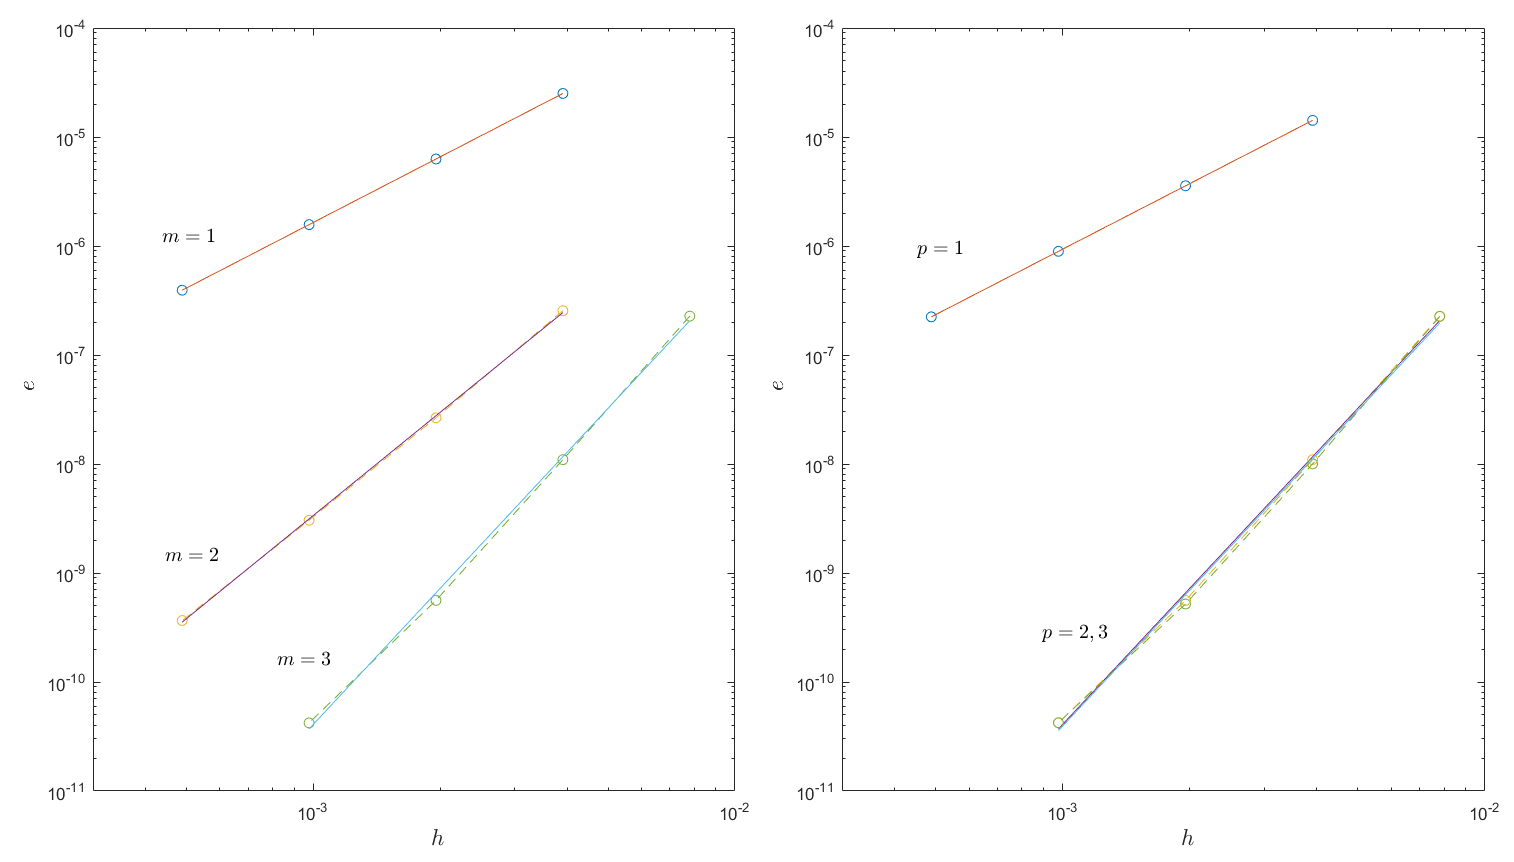
\includegraphics[width=0.95\textwidth]{Graphics/lldp-fj/mp_new.png}}
	\caption{Gráfico Log-log de error ${e_i=\max_{t_n\in(t)_{h_i}}\nnnorm{y_n-x(t_n)}_\infty}$ contra $h_i$ integrando la ecuación de Ejemplo \ref{ex:Brus} con el esquema (\ref{JFLLRK4}), fijados $\eta_1=\eta_2=2$, $\alpha_1=\alpha_2=0.5$, $\beta=1$ y $h_i=2^{-i}$, $i=7,8,9,10,11$, y : Izquierda, $\mf=1,2,3$, $\pf=2$; y Derecha, $\pf=1,2,3$, $\mf=3$.} \label{Fig1}
\end{figure}

\begin{table}[h]
	\centering
	\caption{
		Orden de convergencia $r$ del esquema (\ref{JFLLRK4}) y las estimaciones $\widetilde{r}$ para diferentes valores de $\mf$ y $\pf$, el $90\%$ límite de confianza $\Delta$ de $\widetilde{r}$, y el coeficiente de determinación $R^2$ de la recta ajustada en Figura \ref{Fig1}. Lo valores $\eta_1=\eta_2=2$, $\alpha_1=\alpha_2=0.5$ y $\beta=1$ se mantienen fijos.}
	\begin{adjustbox}{width=0.8\columnwidth,center}
		\begin{tabular}{cccccllccccc}
			\cline{1-12}
			&  & $\pf=2$ &  &  &  &  &  &  & $\mf=3$ &  &  \\ \cline{2-5}\cline{9-12}
			$\mf$ & $r$ & $\widetilde{r}$ & $\pm \varDelta$ & $R^{2}$ &  &  & $\pf+\pf$
			& $r$ & $\widetilde{r}$ & $\pm \varDelta$ & $R^{2}$ \\ 
			\cline{1-5}\cline{8-12}
			1 & 2 & 1.999 & 0.001 & 0.98 &  &  & 2 & 2 & 1.996 & 0.003 & 0.98 \\ 
			2 & 3 & 3.145 & 0.149 & 0.98 &  &  & 4 & 4 & 4.148 & 0.476 & 0.98 \\ 
			3 & 4 & 4.148 & 0.476 & 0.98 &  &  & 6 & 4 & 4.141 & 0.633 & 0.98 \\ 
			\cline{1-12}
		\end{tabular}
	\end{adjustbox}
	\label{tab:mporders}
\end{table}


Los errores $e_i=\max_{t_n\in(t)_{h_i}}\nnnorm{y_n-x(t_n)}_\infty$ del código \textit{JF-LLRK} en la integración de la ecuación de Brusselator fueron calculados para diferentes discretizaciones de tiempo $(t)_{h_i}$ con un tamaño de paso fijo $h_i$, donde la \textquotedblleft solución exacta\textquotedblright ~$x$ se estima mediante el código Matlab \textit{ode15s} con tolerancias $RTol= 10^{-12}$ y $ATol=10^{-14}$. La Figura \ref{Fig1}-izquierda muestra cuatro de estos errores para el código \textit{JF-LLRK} con diferentes valores de $\mf$, y fijo $\pf=2$, $\eta_1=\eta_2=2$ , $\alpha_1=\alpha_2=0.5$ y $\beta=1$, así como la recta ajustada a los puntos $(\log_2(h_i),\log_2(e_i))$ con $i=1,. ..,4$. La tabla \ref{tab:mporders}-izquierda presenta el valor de la pendiente $\widetilde{r}$ de la línea recta ajustada para cada valor de $\mf$, lo que proporciona una estimación del orden de convergencia del esquema. La tabla también presenta los $90\%$ límites de confianza de $\widetilde{r}$, el coeficiente de determinación como indicador de la bondad de la línea ajustada, y el orden de convergencia de convergencia esperado $r$ que - de acuerdo con el Teorema \ref {theorem:kp-fj-llrk-convergence} - el esquema (\ref{JFLLRK4}) tiene para los diferentes valores de $\mf$. La figura \ref{Fig1}-derecha y la tabla \ref{tab:mporders}-derecha presentan salidas similares pero para el código \textit{JF-LLRK} con varios valores de $\pf$ y $\mf=3$ fijados $\eta_1=\eta_2=2$, $\alpha_1=\alpha_2=0.5$ y $\beta=1$. Observe que el orden de convergencia de convergencia estimado $\widetilde{r}$ proporcionada en la Tabla \ref{tab:mporders} está de acuerdo con el orden de convergencia del esquema (\ref{JFLLRK4}) establecido por el Teorema \ref{theorem:kp-fj-llrk-convergence} para los valores considerados de $\mf$ y $\pf$.

Análogamente, las Figuras ref{Fig2}, \ref{Fig3} y las Tablas \ref{tab:out}, \ref{tab:in} presentan los resultados de las simulaciones correspondientes al orden de de convergencia del esquema (\ref{JFLLRK4}) en función de los parámetros de sus dos aproximaciones libres de jacobiano. Nuevamente el orden de convergencia de convergencia estimado $\widetilde{r}$ proporcionada en las tablas \ref{tab:in} y \ref{tab:out} está de acuerdo con el orden de convergencia de convergencia del esquema (\ref{JFLLRK4}) establecido por Teorema \ref{kp-fj-llrk-convergencia} para los valores considerados de $\eta_1$, $\eta_2$, $\alpha_1$, $\alpha_2$ y $\beta$.


\begin{figure}[h]
	\centering
	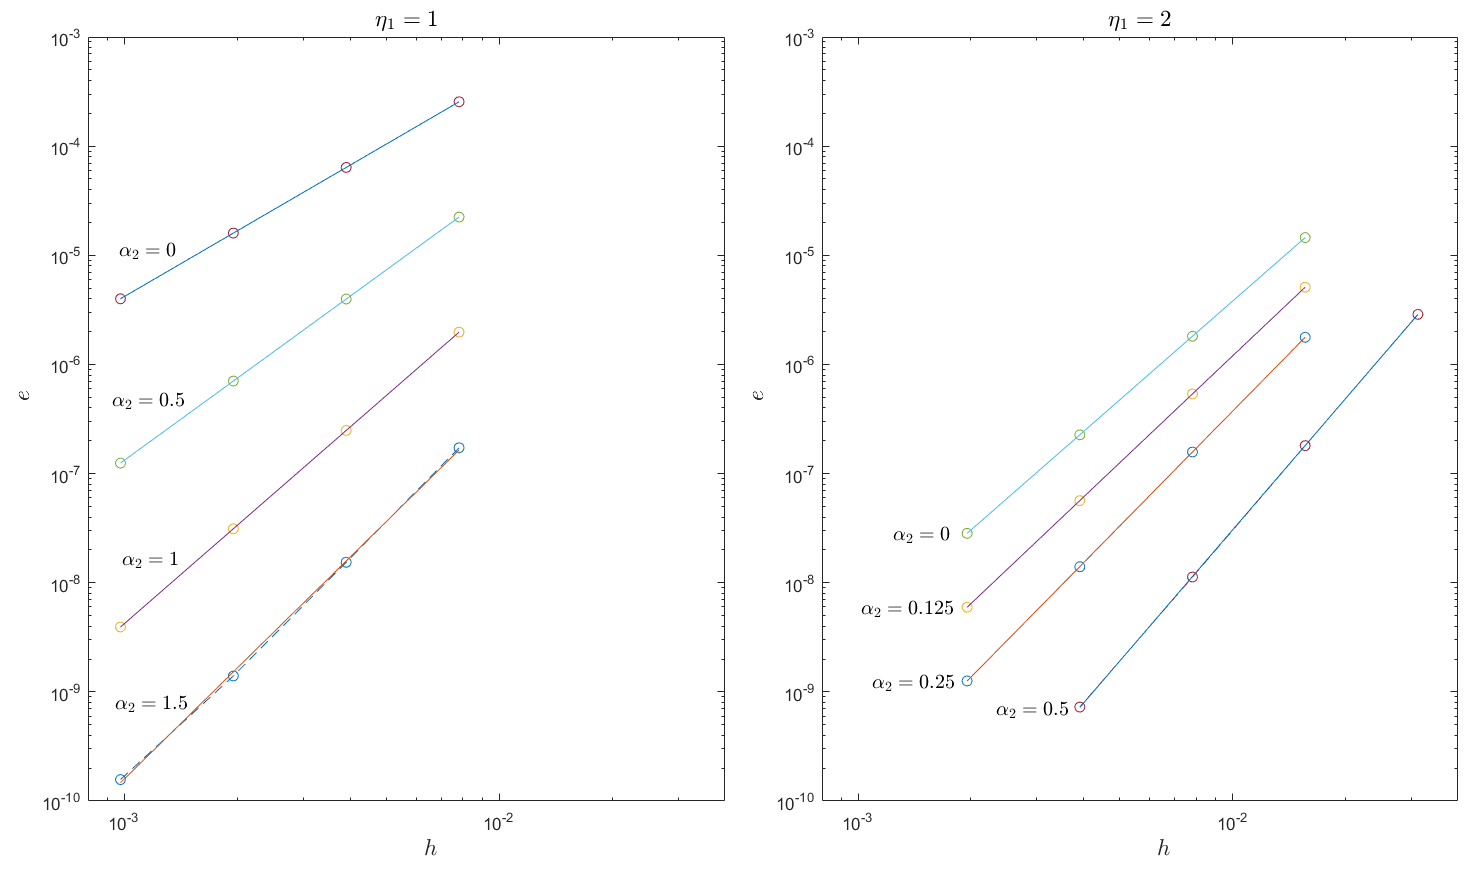
\includegraphics[width=0.95\textwidth]{Graphics/lldp-fj/out_new.png}
	\caption{Gráfico Log-log de error $e_i=\max_{t_n\in(t)_{h_i}}\nnnorm{y_n-x(t_n)}_\infty$ contra $h_i$ integrando la ecuación de Ejemplo \ref{ex:Brus} con el esquema (\ref{JFLLRK4}), fijados $\mf=14$, $\pf=4$, $\eta_1=2$, $\alpha_1=0.5$, $\beta=1$, y: Izquierda, $\eta_2=1$, $\alpha_2=0,0.5,1,1.5$, $h_i=2^{-i}$, $i=7,8,9,10$ y Derecha, $\eta_2=2$, $\alpha_2=0,0.125,0.25,0.5$, $h_i=2^{-i}$, $i=5,6,7,8,9$.}
	\label{Fig2}
\end{figure}

\begin{table}[h]
	\centering
	\caption{
		Orden de convergencia $r$ del esquema (\ref{JFLLRK4}) y las estimaciones $\widetilde{r}$ para diferentes valores de $\eta_2$ y $\alpha_2$, el $90\%$ límite de confianza $\Delta$ de $\widetilde{r}$, el coeficiente de determinación $R^2$ de la recta ajustada en Figura \ref{Fig2}. Los valores de $\mf=14$, $\pf=4$, $\eta_1=2$, $\alpha_1=0.5$ y $\beta=1$ se mantienen fijos. }
	\begin{adjustbox}{width=0.8\columnwidth,center}
		\begin{tabular}{ c  c c c c  c  c c c c c}
			\hline
			& \multicolumn{4}{c}{$\eta_2=1$} & & & \multicolumn{4}{c}{$\eta_2=2$} \\
			\cline{2-5} \cline{8-11}
			$\alpha_2$ & $r$ & $\widetilde{r}$ & $\pm\varDelta$ & $R^2$ & & $\alpha_2$ & $r$ & $\widetilde{r}$ & $\pm\varDelta$ & $R^2$ \\
			\hline
			0 & 2 & 1.999 & 0.001 & 0.98 & & 0 & 3 & 3.000 & 0.002 & 0.97 \\
			0.5 & 2.5 & 2.496 & 0.003 & 0.98 & & 0.125 & 3.25 & 3.247 & 0.003 & 0.97 \\
			1 & 3 & 2.992 & 0.005 & 0.98 & & 0.25 & 3.5 & 3.487 & 0.013 & 0.97 \\
			1.5 & 3.5 & 3.376 & 0.025 & 0.98 & & 0.5 & 4 & 3.986 & 0.029 & 0.97 \\
			\hline
		\end{tabular}
	\end{adjustbox}
	\label{tab:out}
\end{table}


\begin{figure}[h]
	\centering
	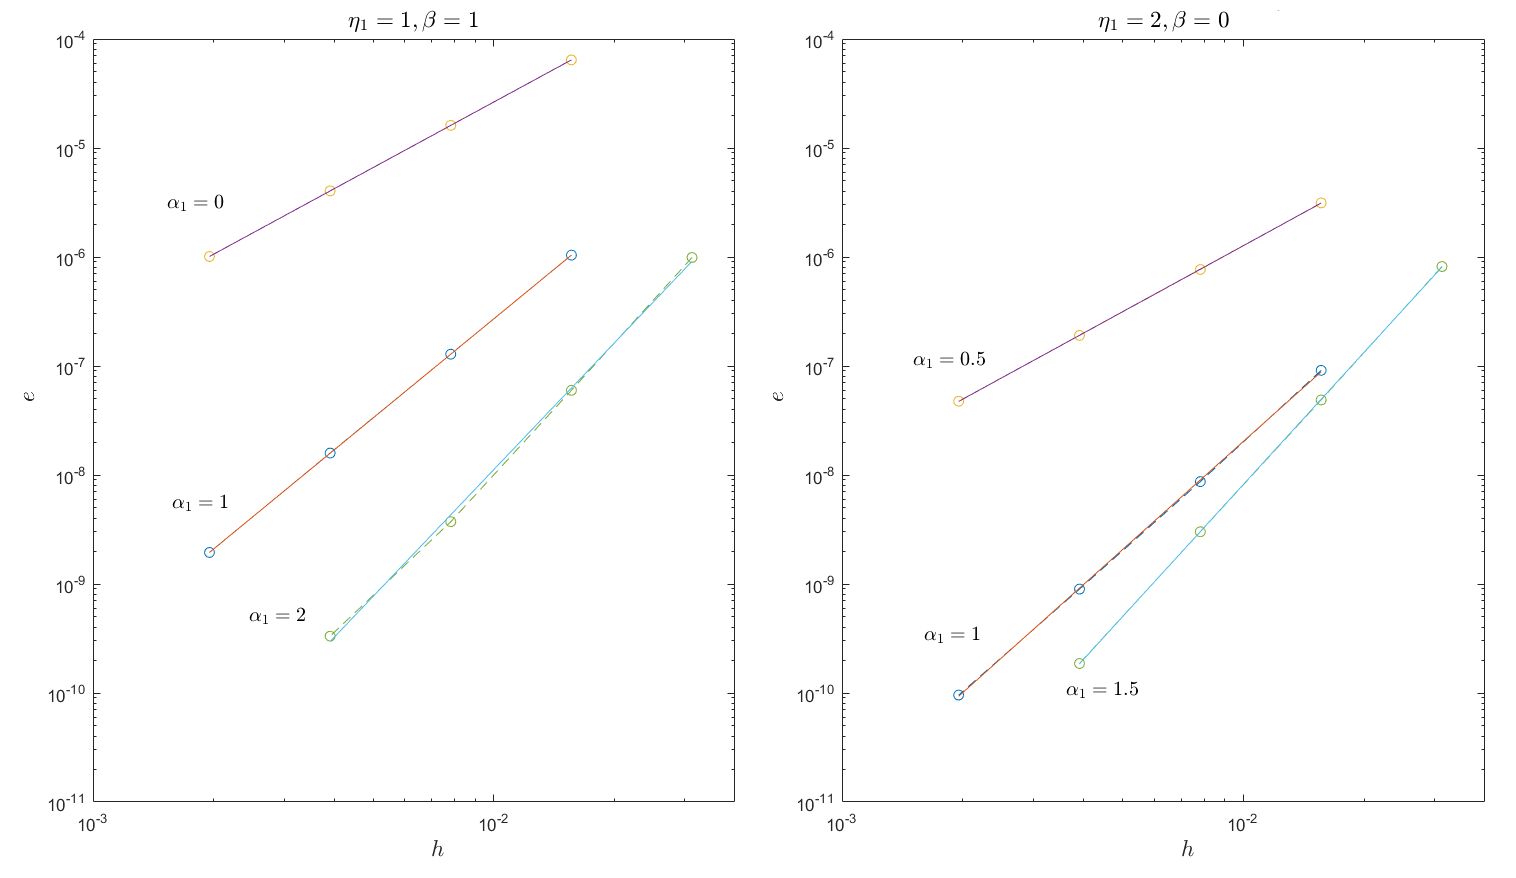
\includegraphics[width=0.95\textwidth]{Graphics/lldp-fj/in_new.png}
	\caption{Gráfico Log-log de error $e_i=\max_{t_n\in(t)_{h_i}}\nnnorm{y_n-x(t_n)}_\infty$ contra $h_i$ integrando la ecuación de Ejemplo \ref{ex:Brus} con el esquema (\ref{JFLLRK4}), fijados $\mf=14$, $\pf=4$, $\eta_2=2$, $\alpha_2=1$, $h_i=2^{-i}$, $i=5,6,7,8,9$, y: Izquierda, $\alpha_1=0,1,2$ for $\eta_1=1,\beta=1$; Derecha, $\alpha_1=0.5,1,1.5$ for $\eta_1=2,\beta=0$.}
	\label{Fig3}
\end{figure}


\begin{table}[h]
	\centering
	\caption{
        Orden de convergencia $r$ del esquema (\ref{JFLLRK4}) y las estimaciones $\widetilde{r}$ para diferentes valores de  $\eta_1$, $\alpha_1$ y $\beta$, el $90\%$ límite de confianza $\Delta$ de $\widetilde{r}$, el coeficiente de determinación $R^2$ de la recta ajustada en Figura \ref{Fig3}. Los valores de $\mf=14$, $\pf=4$, $\eta_2=2$ y$\alpha_2=1$ se mantienen fijos.}
	\begin{adjustbox}{width=0.8\columnwidth,center}
		\begin{tabular}{ccccccccccccc}
			\hline
			&  & \multicolumn{4}{c}{$\eta _{1}=1$} &  &  &  & \multicolumn{4}{c}{$\eta
				_{1}=2$} \\ \cline{3-6}\cline{10-13}
			$\beta $ & $\alpha _{1}$ & $r$ & $\widetilde{r}$ & $\pm \varDelta$ & $R^{2}$
			&  & $\beta $ & $\alpha _{1}$ & $r$ & $\widetilde{r}$ & $\pm \varDelta$ & $%
			R^{2}$ \\ \hline
			1 & 0 & 2 & 1.997 & 0.004 & 0.97 &  & 0 & 0.5 & 2 & 2.014 & 0.017 & 0.97 \\ 
			1 & 1 & 3 & 3.020 & 0.010 & 0.97 &  & 0 & 1 & 3 & 3.300 & 0.116 & 0.97 \\ 
			1 & 2 & 4 & 3.863 & 0.421 & 0.97 &  & 0 & 1.5 & 4 & 4.031 & 0.039 & 0.97 \\ 
			\hline
		\end{tabular}
	\end{adjustbox}
	\label{tab:in}
\end{table}

\subsubsection{Simulaciones comparativas}\label{sc:comparison}

En este conjunto de simulaciones, se utilizaran tres ecuaciones diferenciales parciales empleadas con frecuencia en la literatura como ecuaciones de prueba. Estas ecuaciones son: Brusselator 2D (\ref{ex:Brus}), Brusselator 2D (\ref{ex:Brus2D}), Burger's (\ref{ex:Burger}) y Gray-Scott 2D~(\ref{ex:GS2D}).

Para cada ecuación de prueba, los resultados de la integración numérica se sintetizan en los diagramas de precisión contra tiempo de la Figura \ref{work-precision diagram}. En estos diagramas, la precisión de los códigos \textit{JF-LLRK4}, \textit{JF-Exp4}, \textit{JF-EPIRK4} y \textit{BDF4} se mide por el error $e_i=\max\limits_ {t_n\in(t)_{h_i}}\nnnorm{y_n-x(t_n)}_\infty$ entre la \textquotedblleft solución exacta\textquotedblright~$x$ de la ecuación de prueba y la solución aproximada $y_n$ de cada código calculado en cinco particiones de tiempo con un tamaño de paso fijo $h_i$, donde la \textquotedblleft solución exacta\textquotedblright ~$x $ se estima nuevamente como en las simulaciones preliminares. La figura \ref{work-precision diagram} muestra que, para estas ecuaciones, el esquema LLRK libre de jacobiano (\ref{JFLLRK4}) exhibe una precisión similar o mayor que los otros tres integradores libres de jacobiano, pero con un costo computacional menor o similar. Esta diferencia en el tiempo computacional se explica por los resultados de las Tablas \ref{tab:br}-\ref{tab:gs2d}.

\begin{figure}[h]
	\centering
	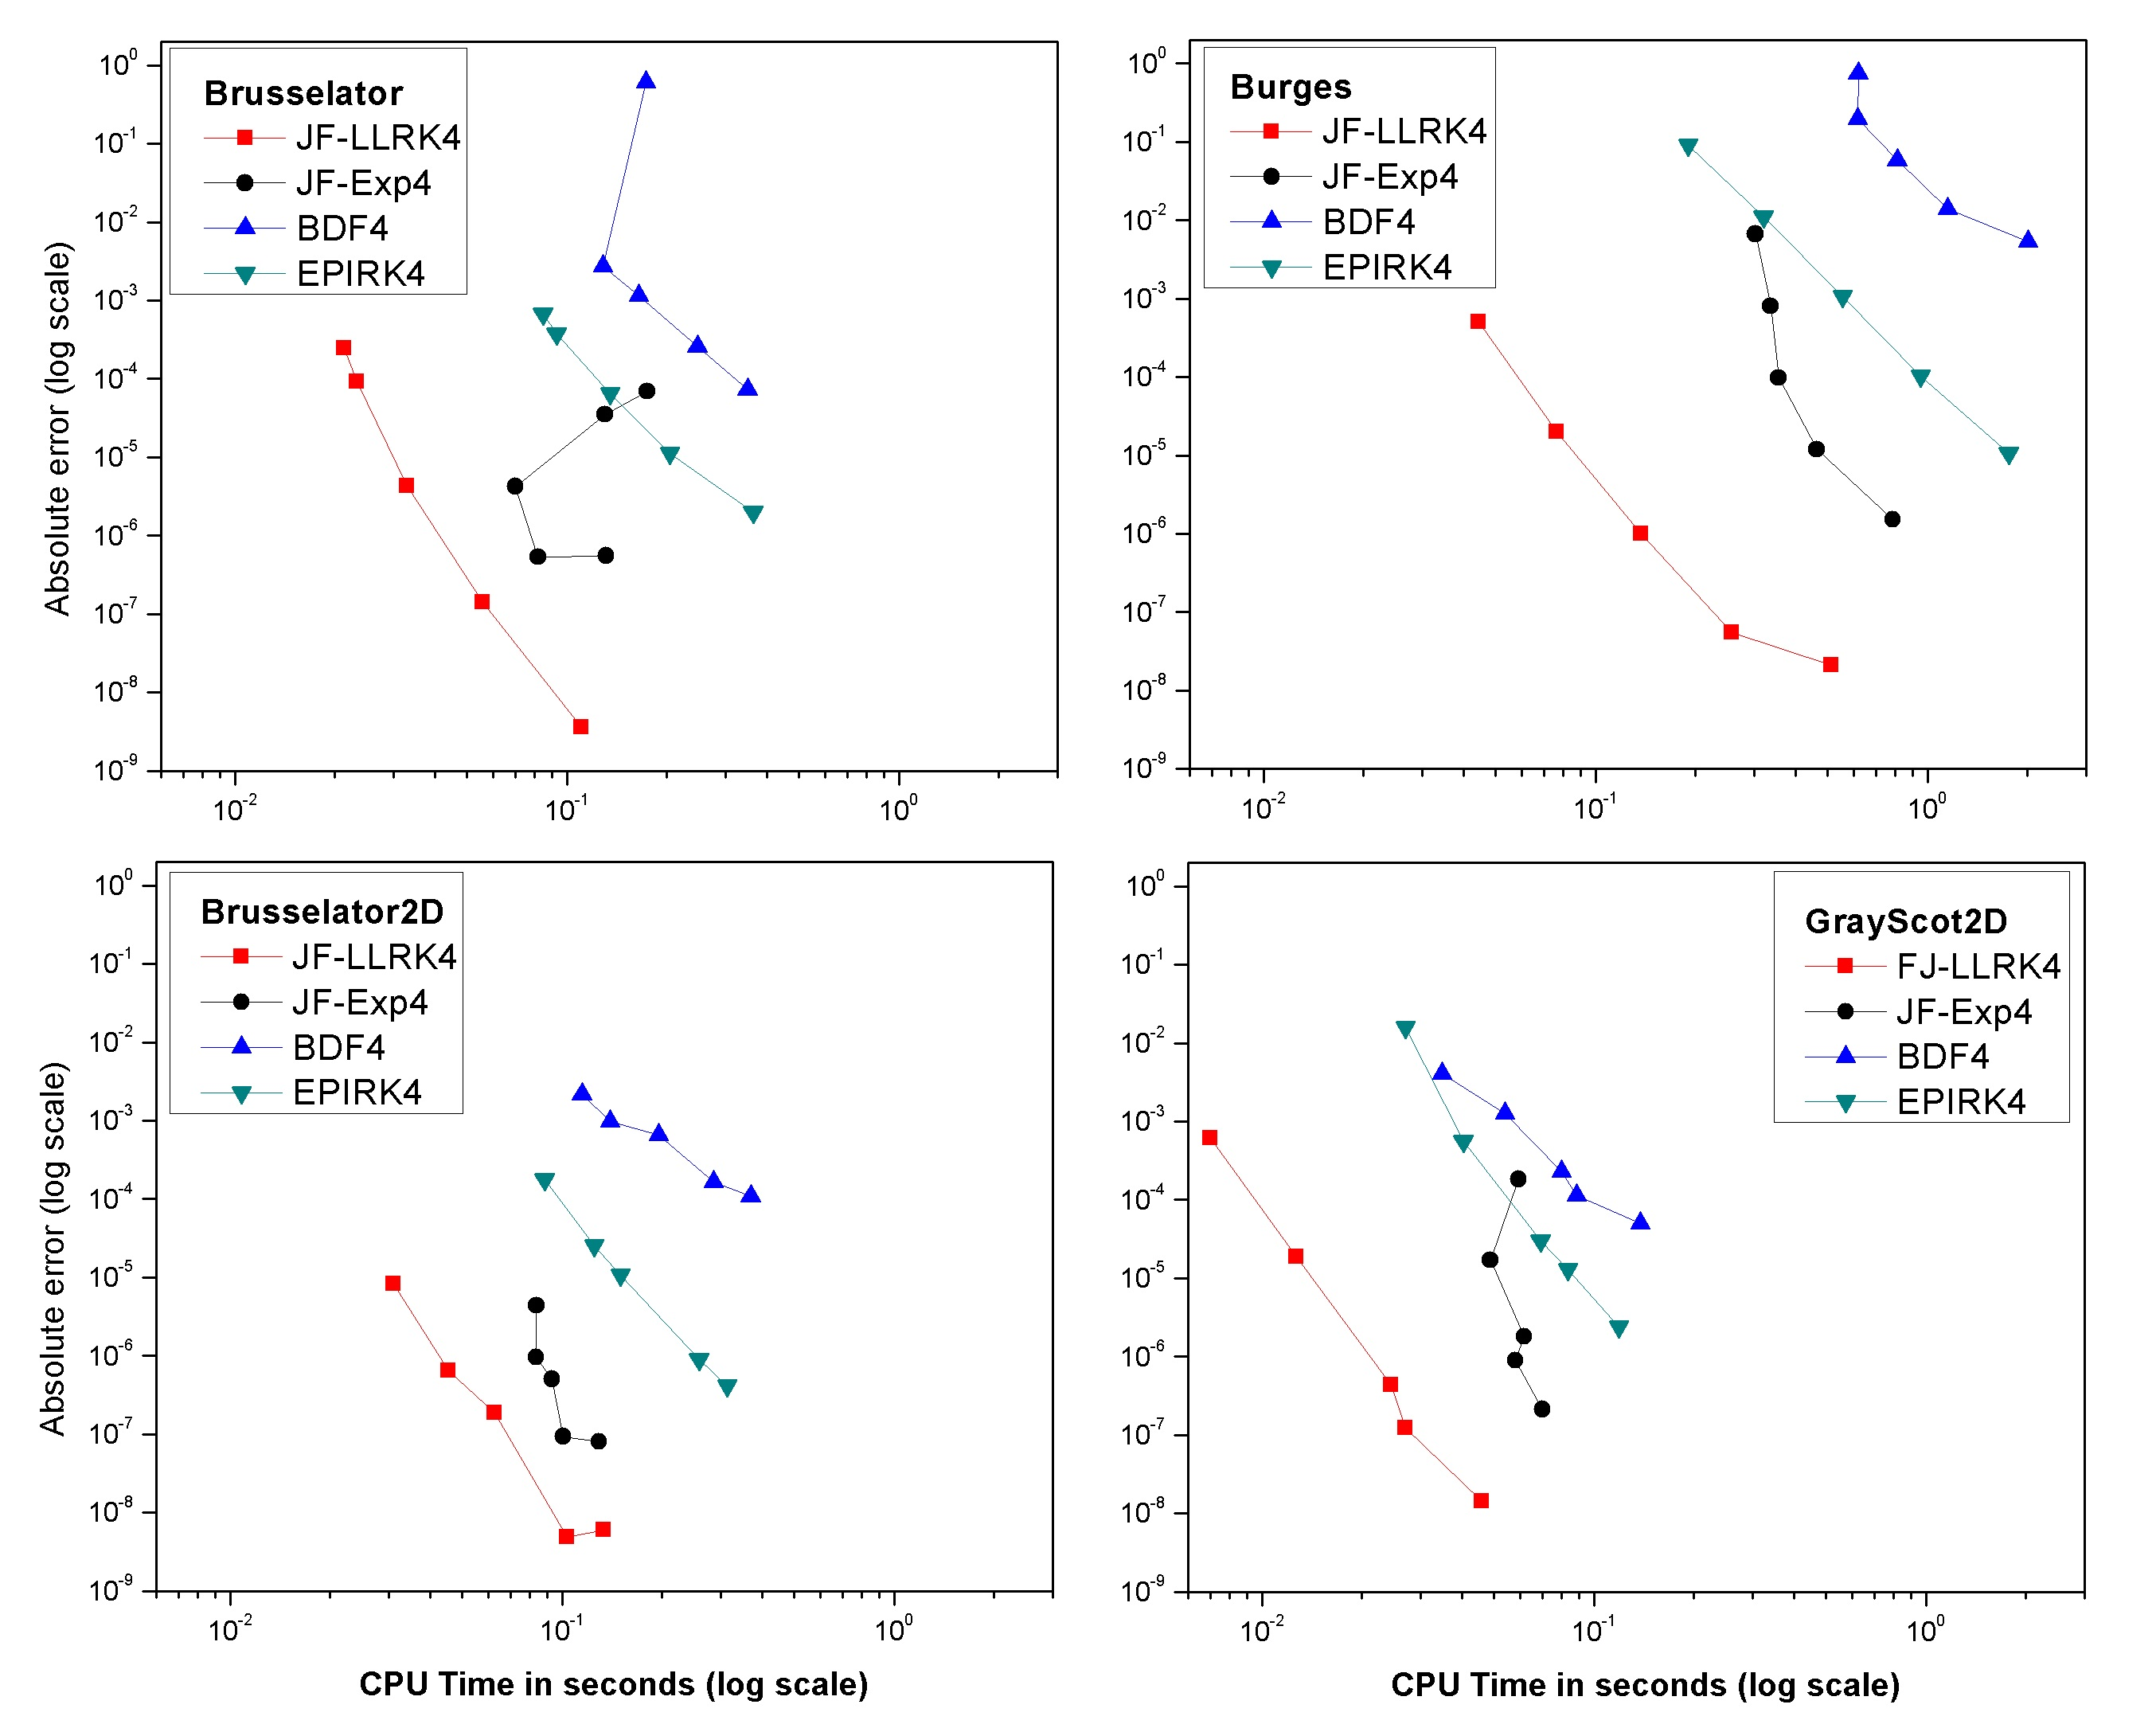
\includegraphics[width=1\textwidth]{Graphics/lldp-fj/Diagram_new.jpg}
	\caption{Diagramas comparativos de precisión contra tiempo en escala log-log para cada uno de los cuatro códigos en la integración delas cuatro ecuaciones de prueba for the four codes in the integration of the four test equations.} \label{work-precision diagram}
\end{figure}

Para cada Código, las Tablas \ref{tab:br}-\ref{tab:gs2d} presentan el tamaño del paso \textit{h}, el número de pasos \textit{Pasos}, el número de evaluaciones del campo vectorial \textit{f-Eval}, el número de aproximaciones del subespacio Krylov \textit{K-subspace} a los productos de la función phi por un vector, el número de sistemas lineales en el código \textit{BDF4} resuelto por el método General Minimal Residue \textit {GMRES}, y el número de aproximaciones de Padé \textit{Padé} requeridas por los tres integradores exponenciales. Además, la dimensión mínima $\mf_{min}$, máxima $\mf_{max}$ y total $\mf_{total}$ de los subespacios de Krylov requerida por los códigos \textit{JF-LLRK4}, \textit{JF -Exp4} y \textit{JF-EPIRK4} para integrar las ecuaciones de prueba en todo el intervalo de integración también se especifica. Para el código \emph{BDF4}, $\mf_{min}$, $\mf_{max}$ y $\mf_{total}$ representan el número mínimo, máximo y total de iteraciones realizadas por el método GMRES sobre el intervalo de integración completo.

En cada paso de integración, al igual que para el esquema (5.8) de \cite{hochbruck1998exponential}, el código \textit{JF-Exp4} realiza tres descomposiciones en subespacios de Krylov y, al menos, tres aproximaciones (6,6)-Padé a la función $\varphi_1$ de las matrices de Hessenberg resultantes del Algoritmo de Arnoldi libre de Jacobiano \ref{alg:iArnoldi}. \textit{JF-Exp4} utiliza la diferencia hacia adelante directa de primer orden como una aproximación del producto de la matriz jacobiana por un vector en el algoritmo \ref{alg:iArnoldi}, lo cual reduce a tres el orden de convergencia del esquema (5.8) de \cite{hochbruck1998exponential} (ver Teorema 5.1 en \cite{hochbruck1998exponential}). Para estimar la dimensión de Krylov $\mf$, el código \textit{JF-Exp4} usa el algoritmo adaptativo de \cite{hochbruck1998exponential} y no hay restricción al valor mínimo para $\mf$.

El código \textit{JF-EPIRK4} requiere de las mismas descomposiciones de Krylov y un número similar de aproximaciones de Padé que el código \textit{JF-Exp4} en cada paso de integración, pero la dimensión de Krylov $\mf$ se estima automáticamente mediante el estrategia adaptativa de \cite{niesen2012algorithm} implementada en el código de Matlab \textit{phipm}.

Para resolver los sistemas algebraicos no lineales, en cada paso de integración, el código \textit{BDF4} emplea el método clásico de Newton junto con el método General Minimal Residue (GMRES) (función de Matlab \textit{gmres} con tolerancia $RTol=10^{-6}$) y la diferencia finita hacia adelante de primer orden como una aproximación al producto de la matriz jacobiana pro un vector. En la función de Matlab \textit{gmres}, se eliminaron las comprobaciones computacionalmente costosas de las funciones de Matlab \textit{iterchk} y \textit{iterapp}.

\begin{table}[h!]
	\caption{Desempeño de los códigos en la integración de la ecuación Brusselator con $M=100$, $d=200$.}
	\centering
	\begin{adjustbox}{width=0.9\columnwidth,center}
		\begin{tabular}{cccccccccc}
			\hline
			\textit{h} & Código & Pasos & f-Eval & K-subspace & GMRES & Padé & $\mf_{total}$ & $\mf%
			_{min}$ & $\mf_{max}$ \\ \hline
			\multicolumn{1}{l}{0.0250} & \multicolumn{1}{l}{JF-LLRK4} & 40 & 852 & 40 &
			0 & 40 & 492 & 4 & 16 \\
			\multicolumn{1}{l}{} & \multicolumn{1}{l}{JF-Exp4} & 40 & 3324 & 120 & 0 &
			1168 & 3124 & 4 & 48 \\
			\multicolumn{1}{l}{} & \multicolumn{1}{l}{BDF4} & 40 & 7318 & 0 & 400 & 0 &
			3305 & 3 & 24 \\
			\multicolumn{1}{l}{} & \multicolumn{1}{l}{JF-EPIRK4} & 40 & 1238 & 120 & 0 &
			625 & 718 & 4 & 11 \\
			\multicolumn{1}{l}{0.0200} & \multicolumn{1}{l}{JF-LLRK4} & 50 & 967 & 50 &
			0 & 50 & 517 & 4 & 13 \\
			\multicolumn{1}{l}{} & \multicolumn{1}{l}{JF-Exp4} & 50 & 2855 & 150 & 0 &
			1147 & 2605 & 4 & 48 \\
			\multicolumn{1}{l}{} & \multicolumn{1}{l}{BDF4} & 50 & 7156 & 0 & 448 & 0 &
			2780 & 2 & 23 \\
			\multicolumn{1}{l}{} & \multicolumn{1}{l}{JF-EPIRK4} & 50 & 1425 & 150 & 0 &
			716 & 775 & 3 & 10 \\
			\multicolumn{1}{l}{0.0100} & \multicolumn{1}{l}{JF-LLRK4} & 100 & 1477 & 100
			& 0 & 100 & 577 & 4 & 10 \\
			\multicolumn{1}{l}{} & \multicolumn{1}{l}{JF-Exp4} & 100 & 1773 & 300 & 0 &
			970 & 1273 & 2 & 36 \\
			\multicolumn{1}{l}{} & \multicolumn{1}{l}{BDF4} & 100 & 6574 & 0 & 476 & 0 &
			2269 & 2 & 13 \\
			\multicolumn{1}{l}{} & \multicolumn{1}{l}{JF-EPIRK4} & 100 & 2278 & 300 & 0 &
			976 & 978 & 2 & 7 \\
			\multicolumn{1}{l}{0.0050} & \multicolumn{1}{l}{JF-LLRK4} & 200 & 2609 & 200
			& 0 & 200 & 809 & 4 & 6 \\
			\multicolumn{1}{l}{} & \multicolumn{1}{l}{JF-Exp4} & 200 & 2256 & 600 & 0 &
			1242 & 1256 & 1 & 15 \\
			\multicolumn{1}{l}{} & \multicolumn{1}{l}{BDF4} & 200 & 7055 & 0 & 588 & 0 &
			2678 & 1 & 12 \\
			\multicolumn{1}{l}{} & \multicolumn{1}{l}{JF-EPIRK4} & 200 & 3894 & 600 & 0 &
			1294 & 1294 & 1 & 5 \\
			\multicolumn{1}{l}{0.0025} & \multicolumn{1}{l}{JF-LLRK4} & 400 & 5201 & 400
			& 0 & 400 & 1601 & 4 & 5 \\
			\multicolumn{1}{l}{} & \multicolumn{1}{l}{JF-Exp4} & 400 & 3945 & 1200 & 0 &
			1945 & 1945 & 1 & 4 \\
			\multicolumn{1}{l}{} & \multicolumn{1}{l}{BDF4} & 400 & 9530 & 0 & 919 & 0 &
			3556 & 1 & 10 \\
			\multicolumn{1}{l}{} & \multicolumn{1}{l}{JF-EPIRK4} & 400 & 7287 & 1200 & 0 &
			2087 & 2087 & 1 & 3 \\
			\hline
		\end{tabular}
	\end{adjustbox}
	\label{tab:br}
\end{table}



\begin{table}[h!]
	\caption{Desempeño de los códigos en la integración de la ecuación Brusselator 2D con $M=40$, $d=3200$.}
	\centering
	\begin{adjustbox}{width=0.9\columnwidth,center}
		\begin{tabular}{cccccccccc}
			\hline
			\textit{h} & Código & Pasos & f-Eval & K-subspace & GMRES & Padé & $\mf_{total}$ & $\mf%
			_{min}$ & $\mf_{max}$ \\ \hline
			\multicolumn{1}{l}{0.01000} & \multicolumn{1}{l}{JF-LLRK4} & 10 & 144 & 10
			& 0 & 10 & 54 & 4 & 8 \\
			\multicolumn{1}{l}{} & \multicolumn{1}{l}{JF-Exp4} & 10 & 251 & 30 & 0 & 139
			& 201 & 2 & 20 \\
			\multicolumn{1}{l}{} & \multicolumn{1}{l}{BDF4} & 10 & 1243 & 0 & 86 & 0 &
			283 & 2 & 8 \\
			\multicolumn{1}{l}{} & \multicolumn{1}{l}{JF-EPIRK4} & 10 & 263 & 30 & 0 &
			129 & 133 & 3 & 6 \\
			\multicolumn{1}{l}{0.00625} & \multicolumn{1}{l}{JF-LLRK4} & 16 & 218 & 16
			& 0 & 16 & 74 & 4 & 6 \\
			\multicolumn{1}{l}{} & \multicolumn{1}{l}{JF-Exp4} & 16 & 284 & 48 & 0 & 167
			& 204 & 2 & 15 \\
			\multicolumn{1}{l}{} & \multicolumn{1}{l}{BDF4} & 16 & 1618 & 0 & 118 & 0 &
			334 & 1 & 7 \\
			\multicolumn{1}{l}{} & \multicolumn{1}{l}{JF-EPIRK4} & 16 & 383 & 48 & 0 &
			174 & 175 & 2 & 6 \\
			\multicolumn{1}{l}{0.00500} & \multicolumn{1}{l}{JF-LLRK4} & 20 & 268 & 20 &
			0 & 20 & 88 & 4 & 6 \\
			\multicolumn{1}{l}{} & \multicolumn{1}{l}{JF-Exp4} & 20 & 307 & 60 & 0 & 184
			& 207 & 2 & 15 \\
			\multicolumn{1}{l}{} & \multicolumn{1}{l}{BDF4} & 20 & 1449 & 0 & 109 & 0 &
			313 & 1 & 6 \\
			\multicolumn{1}{l}{} & \multicolumn{1}{l}{JF-EPIRK4} & 20 & 464 & 60 & 0 &
			204 & 204 & 2 & 5 \\
			\multicolumn{1}{l}{0.00250} & \multicolumn{1}{l}{JF-LLRK4} & 40 & 521 & 40 &
			0 & 40 & 161 & 4 & 5 \\
			\multicolumn{1}{l}{} & \multicolumn{1}{l}{JF-Exp4} & 40 & 455 & 120 & 0 & 251
			& 255 & 1 & 8 \\
			\multicolumn{1}{l}{} & \multicolumn{1}{l}{BDF4} & 40 & 1452 & 0 & 120 & 0 &
			384 & 1 & 5 \\
			\multicolumn{1}{l}{} & \multicolumn{1}{l}{JF-EPIRK4} & 40 & 846 & 120 & 0 &
			326 & 326 & 1 & 4 \\
			\multicolumn{1}{l}{0.00200} & \multicolumn{1}{l}{JF-LLRK4} & 50 & 650 & 50
			& 0 & 50 & 200 & 4 & 4 \\
			\multicolumn{1}{l}{} & \multicolumn{1}{l}{JF-Exp4} & 50 & 541 & 150 & 0 & 289
			& 291 & 1 & 8 \\
			\multicolumn{1}{l}{} & \multicolumn{1}{l}{BDF4} & 50 & 1785 & 0 & 150 & 0 &
			457 & 1 & 5 \\
			\multicolumn{1}{l}{} & \multicolumn{1}{l}{JF-EPIRK4} & 50 & 1027 & 150 & 0 &
			377 & 377 & 1 & 4 \\
			\hline
		\end{tabular}
	\end{adjustbox}
	\label{tab:br2d}
\end{table}

\begin{table}[h!]
	\caption{Desempeño de los códigos en la integración de la ecuación Burger's con $M=400$, $d=400$.}
	\centering
	\begin{adjustbox}{width=0.9\columnwidth,center}
		\begin{tabular}{cccccccccc}
			\hline
			\textit{h} & Código & Pasos & f-Eval & K-subspace & GMRES & Padé & $\mf_{total}$ & $\mf%
			_{min}$ & $\mf_{max}$ \\ \hline
			\multicolumn{1}{l}{0.0050000} & \multicolumn{1}{l}{JF-LLRK4} & 100 & 1614 &
			100 & 0 & 100 & 714 & 4 & 10 \\
			\multicolumn{1}{l}{} & \multicolumn{1}{l}{JF-Exp4} & 100 & 6104 & 300 & 0 &
			2507 & 5604 & 3 & 27 \\
			\multicolumn{1}{l}{} & \multicolumn{1}{l}{BDF4} & 100 & 17304 & 0 & 910 & 0
			& 6469 & 2 & 12 \\
			\multicolumn{1}{l}{} & \multicolumn{1}{l}{JF-EPIRK4} & 100 & 2874 & 300 & 0 &
			1435 & 1574 & 3 & 7 \\
			\multicolumn{1}{l}{0.0025000} & \multicolumn{1}{l}{JF-LLRK4} & 200 & 2922 &
			200 & 0 & 200 & 1122 & 4 & 8 \\
			\multicolumn{1}{l}{} & \multicolumn{1}{l}{JF-Exp4} & 200 & 7287 & 600 & 0 &
			3784 & 6287 & 2 & 20 \\
			\multicolumn{1}{l}{} & \multicolumn{1}{l}{BDF4} & 200 & 27333 & 0 & 1665 & 0
			& 7783 & 2 & 10 \\
			\multicolumn{1}{l}{} & \multicolumn{1}{l}{JF-EPIRK4} & 200 & 4988 & 600 & 0 &
			2388 & 2388 & 2 & 5 \\
			\multicolumn{1}{l}{0.0012500} & \multicolumn{1}{l}{JF-LLRK4} & 400 & 5361 &
			400 & 0 & 400 & 1761 & 4 & 5 \\
			\multicolumn{1}{l}{} & \multicolumn{1}{l}{JF-Exp4} & 400 & 8123 & 1200 & 0 &
			4975 & 6123 & 1 & 11 \\
			\multicolumn{1}{l}{} & \multicolumn{1}{l}{BDF4} & 400 & 37402 & 0 & 2454 & 0
			& 9416 & 2 & 10 \\
			\multicolumn{1}{l}{} & \multicolumn{1}{l}{JF-EPIRK4} & 400 & 9111 & 1200 & 0 &
			3911 & 3911 & 1 & 4 \\
			\multicolumn{1}{l}{0.0006250} & \multicolumn{1}{l}{JF-LLRK4} & 800 & 10400 &
			800 & 0 & 800 & 3200 & 4 & 4 \\
			\multicolumn{1}{l}{} & \multicolumn{1}{l}{JF-Exp4} & 800 & 11223 & 2400 & 0
			& 7039 & 7223 & 1 & 8 \\
			\multicolumn{1}{l}{} & \multicolumn{1}{l}{BDF4} & 800 & 32269 & 0 & 2251 & 0
			& 8838 & 2 & 5 \\
			\multicolumn{1}{l}{} & \multicolumn{1}{l}{JF-EPIRK4} & 800 & 16766 & 2400 & 0 &
			6366 & 6366 & 1 & 4 \\
			\multicolumn{1}{l}{0.0003125} & \multicolumn{1}{l}{JF-LLRK4} & 1600 & 20800
			& 1600 & 0 & 1600 & 6400 & 4 & 4 \\
			\multicolumn{1}{l}{} & \multicolumn{1}{l}{JF-Exp4} & 1600 & 19555 & 4800 & 0
			& 11555 & 11555 & 1 & 4 \\
			\multicolumn{1}{l}{} & \multicolumn{1}{l}{BDF4} & 1600 & 58643 & 0 & 4360 & 0
			& 17910 & 2 & 8 \\
			\multicolumn{1}{l}{} & \multicolumn{1}{l}{JF-EPIRK4} & 1600 & 31872 & 4800 & 0 &
			11072 & 11072 & 1 & 3 \\
			\hline
		\end{tabular}
	\end{adjustbox}
	\label{tab:bg}
\end{table}


\begin{table}[h!]
	\caption{Desempeño de los códigos en la integración de la ecuación Gray-Scott 2D con $M=20$, $d=800$.}
	\centering
	\begin{adjustbox}{width=0.9\columnwidth,center}
		\begin{tabular}{cccccccccc}
			\hline
			\textit{h} & Código & Pasos & f-Eval & K-subspace & GMRES & Padé & $\mf_{total}$ & $\mf%
			_{min}$ & $\mf_{max}$ \\ \hline
			0.010000 & \multicolumn{1}{l}{JF-LLRK4} & 10 & 161 & 10 & 0 & 10 & 71 & 4 &
			10 \\
			& \multicolumn{1}{l}{JF-Exp4} & 10 & 656 & 30 & 0 & 258 & 606 & 4 & 36 \\
			& \multicolumn{1}{l}{BDF4} & 10 & 923 & 0 & 52 & 0 & 332 & 2 & 14 \\
			& \multicolumn{1}{l}{JF-EPIRK4} & 10 & 296 & 30 & 0 & 148 & 166 & 4 & 9 \\
			0.005000 & \multicolumn{1}{l}{JF-LLRK4} & 20 & 296 & 20 & 0 & 20 & 116 & 4 &
			8 \\
			& \multicolumn{1}{l}{JF-Exp4} & 20 & 643 & 60 & 0 & 327 & 543 & 2 & 27 \\
			& \multicolumn{1}{l}{BDF4} & 20 & 1064 & 0 & 72 & 0 & 371 & 1 & 10 \\
			& \multicolumn{1}{l}{JF-EPIRK4} & 20 & 494 & 60 & 0 & 228 & 234 & 2 & 7 \\
			0.002500 & \multicolumn{1}{l}{JF-LLRK4} & 40 & 547 & 40 & 0 & 40 & 187 & 4 &
			8 \\
			& \multicolumn{1}{l}{JF-Exp4} & 40 & 787 & 120 & 0 & 439 & 587 & 1 & 20 \\
			& \multicolumn{1}{l}{BDF4} & 40 & 1308 & 0 & 101 & 0 & 468 & 2 & 7 \\
			& \multicolumn{1}{l}{JF-EPIRK4} & 40 & 889 & 120 & 0 & 369 & 369 & 1 & 5 \\
			0.002000 & \multicolumn{1}{l}{JF-LLRK4} & 50 & 669 & 50 & 0 & 50 & 219 & 4 &
			6 \\
			& \multicolumn{1}{l}{JF-Exp4} & 50 & 876 & 150 & 0 & 488 & 626 & 1 & 15 \\
			& \multicolumn{1}{l}{BDF4} & 50 & 1472 & 0 & 118 & 0 & 528 & 2 & 7 \\
			& \multicolumn{1}{l}{JF-EPIRK4} & 50 & 1079 & 150 & 0 & 429 & 429 & 1 & 5 \\
			0.001250 & \multicolumn{1}{l}{JF-LLRK4} & 80 & 1050 & 80 & 0 & 80 & 330 & 4
			& 6 \\
			& \multicolumn{1}{l}{JF-Exp4} & 80 & 1118 & 240 & 0 & 619 & 718 & 1 & 15 \\
			& \multicolumn{1}{l}{BDF4} & 80 & 2151 & 0 & 184 & 0 & 715 & 1 & 6 \\
			& \multicolumn{1}{l}{JF-EPIRK4} & 80 & 1626 & 240 & 0 & 586 & 586 & 1 & 4 \\
			\hline
		\end{tabular}
	\end{adjustbox}
	\label{tab:gs2d}
\end{table}


Se puede observar de las Tablas \ref{tab:br}-\ref{tab:gs2d}, que el código \textit{BDF4} requiere de un número mucho mayor de evaluaciones del campo vectorial que los otros tres códigos, lo que explica su mayor costo computacional en los diagramas de precisión contra tiempo de la Figura \ref{work-precision diagram}. Por otro lado, para los tamaños de paso más grandes, el número de evaluaciones del campo vectorial de los códigos \textit{JF-Exp4} y \textit{JF-EPIRK4} es mayor que el del código \textit{JF-LLRK4}, por lo que su costo computacional es mucho mayor que el del código \textit{JF-LLRK4}. Para los tamaños de paso más pequeños, el número de evaluaciones del campo vectorial del código \textit{JF-Exp4} es ligeramente inferior o similar al del código \textit{JF-LLRK4}, lo que explica el costo computacional similar de estos dos códigos. En la parte inferior de los diagramas de precisión contra tiempo de la Figura \ref{work-precision diagram} correspondientes a las ecuaciones Brusselator y Brusselator 2D.

Además, las Tablas \ref{tab:br}-\ref{tab:gs2d} muestran la efectividad de la estrategia del código \textit{JF-LLRK4} para la selección de la dimensión Krylov $\mf$ en cada paso de integración, con mínima variación entre los valores de $\mf_{min}$ y $\mf_{max}$, y por tanto, con un valor de $\mf_{total}$ mucho menor que los demás códigos.

En resumen, las simulaciones han demostrado que, con un costo computacional similar, el nuevo integrador libre de jacobiano presenta una precisión mucho mayor que los otros tres integradores libres de jacobiano; mientras que, con una precisión similar, el primero es mucho más rápido que los segundos.

Para concluir esta sección, recordemos que la selección de $\delta$ y $h$ en esquemas prácticos libres de jacobiano se realiza bajo diferentes criterios que resultan en valores óptimos para $\delta$ y $h$ independientes entre sí \cite{knoll2004jacobian}. Con este conocimiento en mente, la teoría desarrollada hasta este punto y los experimentos numéricos realizados con $\delta$ vinculados a una potencia de $h$ pretenden sentar las bases para diseñar esquemas prácticos Localmente Linealizados de Orden Superior Libres Jacobiano con valores óptimos de $h$ y $\delta$.